\documentclass[
	letterpaper, % Paper size, specify a4paper (A4) or letterpaper (US letter)
	12pt, % Default font size, specify 10pt, 11pt or 12pt
]{CSUniSchoolLabReport}

\usepackage{fancyvrb}

\title{Analyzing relation between voltage and current in a simulation.}

\author{Sebastien \textsc{Psarianos}}

\date{\today}


\begin{document}

\maketitle

\begin{center}
	\begin{tabular}{l r}
		Date Performed: & September 13, 2022 \\
	\end{tabular}
\end{center}


\section{Introduction}
The purpose of this experiment is to measure the relationship between current and voltage by determining the resistance of an unknown resistor using a linear fit. Ohm's Law is used to relate the current and voltage to the resistance. This experiment was conducted in the circuit simulator located at:
\begin{verbatim}
	https://phet.colorado.edu/sims/html/
	circuit-construction-kit-dc-virtual-lab/latest/
	circuit-construction-kit-dc-virtual-lab_en.html
\end{verbatim}
There were two resistors used in this experiment and the experiment is divided into three sections.\\

Experiment 1 (1st resistor): Resistor 1 is connected in series with a battery without any wire resistance. Multiple voltage measurements are taken at various battery voltages of the potential difference across the resistor as well as the current through the circuit.\\

Experiment 2 (2nd Resistor): Experiment 1 is repeated with the second resistor.\\

Experiment 3 (2nd Resistor): Resistor 2 is connected in series with a battery with wires that have wire resistance. The unknown resistor in this experiment the sum of all the wire resistance in the circuit. Multiple measurements are taken of the potential difference across the battery as well as the circuit current.\\

\section{Theory}
Two equations are used in the calculations in this lab:\\
\textbf{Ohm's Law} (Equation 1): $\Delta V = IR$\\
\textbf{Kirchoff's Loop Law} (Equation 2): $\Delta V_{circuit} = 0$


\section{Experimental Setup}
The following are images of the apparatus for each experiment:
\begin{center}
    \textbf{Figure 3.1: Experiment 1 Apparatus}\\
    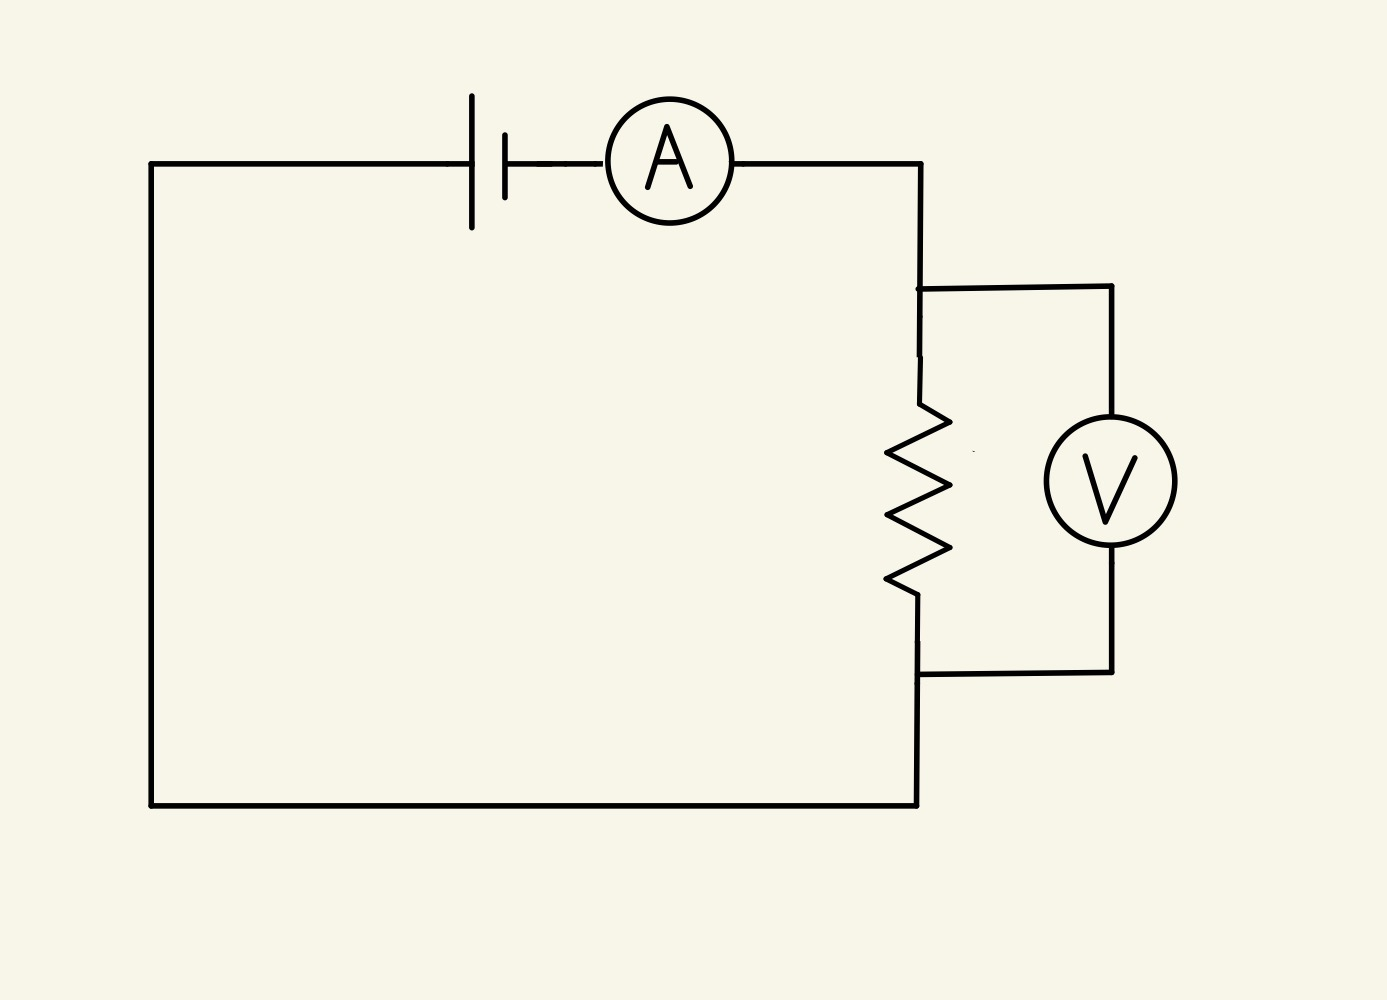
\includegraphics[width=0.65\textwidth]{experimentOneApparatus}
\end{center}
\begin{center}
    \textbf{Figure 3.2: Experiment 2 Apparatus}\\
    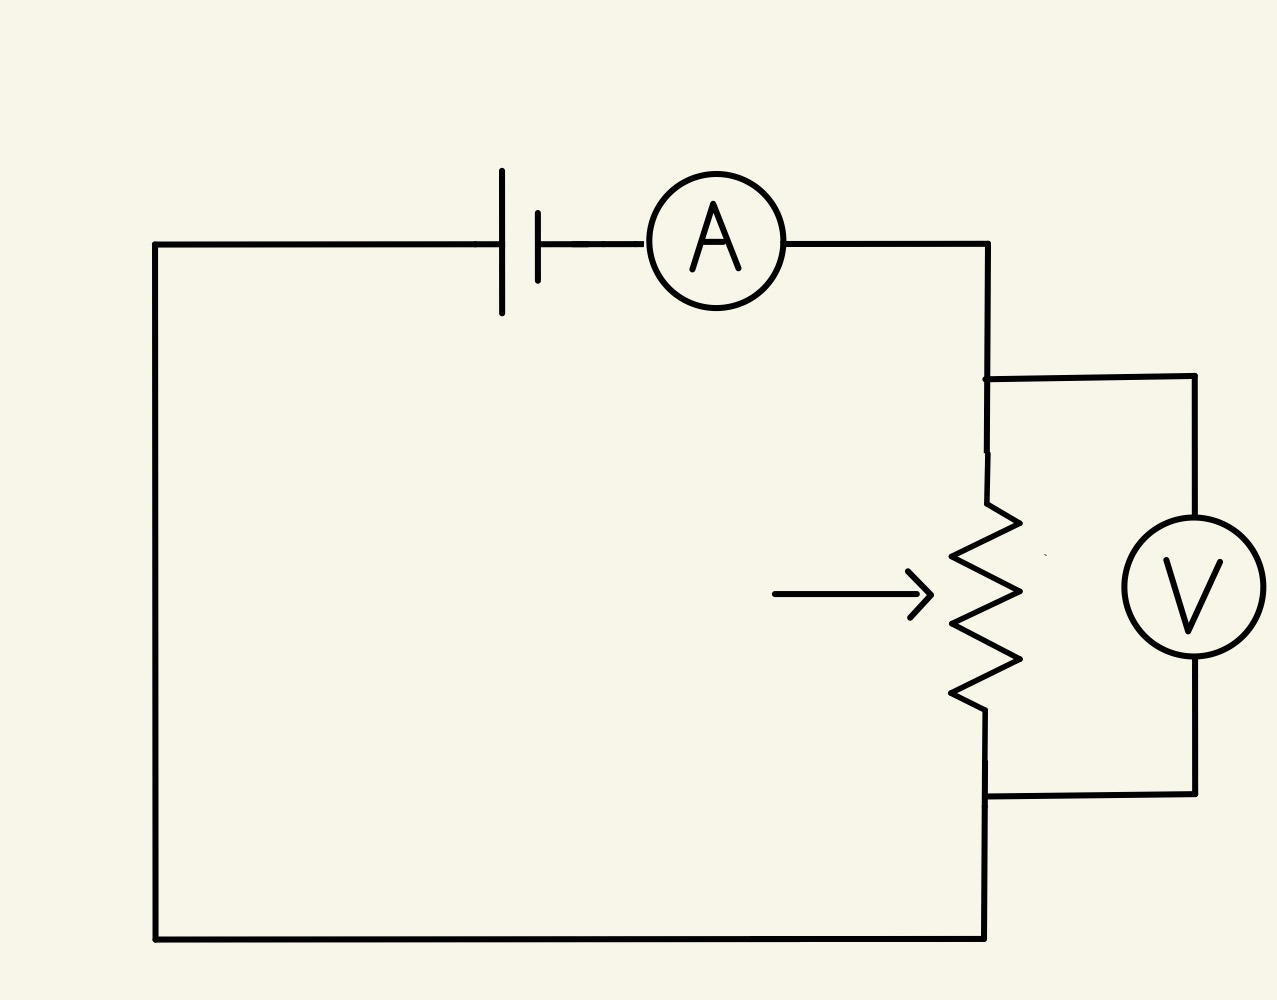
\includegraphics[width=0.65\textwidth]{experimentTwoApparatus}
\end{center}
\begin{center}
    \textbf{Figure 3.3: Experiment 3 Apparatus}\\
    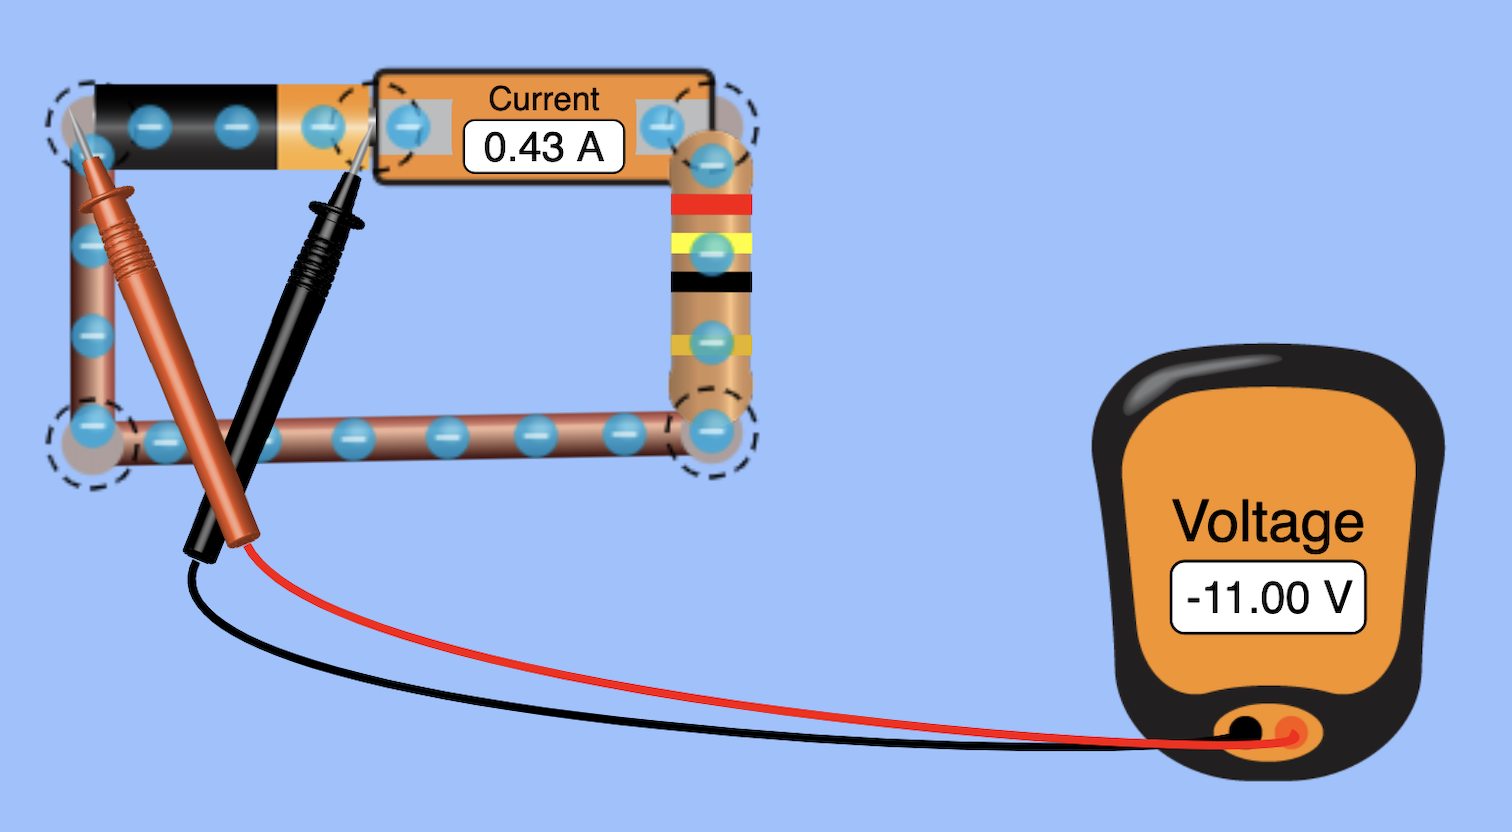
\includegraphics[width=0.65\textwidth]{experimentThreeApparatus}
\end{center}

\section{Results}

\begin{center}
    \textbf{Figure 4.1: Experiment 1 Raw Data}
\end{center}
\setlength\arrayrulewidth{2pt}
\begin{center}
\begin{tabular}{  | l | l | }
	\hline
	Resistor $\Delta V$ (Volts) & Current (Amps) \\
	\hline
	$11.00\pm0.03$& $1.100\pm0.01$\\
	$10.00\pm0.03$& $1.000\pm0.01$\\
	$9.00\pm0.02$& $0.900\pm0.01$\\
	$8.00\pm0.02$& $0.800\pm0.01$\\
	$7.00\pm0.02$& $0.700\pm0.01$\\
	$6.00\pm0.02$& $0.600\pm0.01$\\
	$5.00\pm0.02$& $0.500\pm0.01$\\
	\hline
\end{tabular}
\end{center}



\begin{center}
	\textbf{Figure 4.2: Experiment 2 Raw Data}
\end{center}
\begin{center}
	\begin{tabular}{  | l | l | }
		\hline
		Resistor $\Delta V$ (Volts) & Current (Amps) \\
		\hline
		$11.00\pm0.03$& $0.470\pm0.01$\\
		$10.00\pm0.03$& $0.420\pm0.01$\\
		$9.00\pm0.02$& $0.380\pm0.01$\\
		$8.00\pm0.02$& $0.340\pm0.01$\\
		$7.00\pm0.02$& $0.300\pm0.01$\\
		$6.00\pm0.02$& $0.250\pm0.01$\\
		$5.00\pm0.02$& $0.210\pm0.01$\\
		\hline
	\end{tabular}
\end{center}


\begin{center}
	\textbf{Figure 4.3: Experiment 3 Raw Data}
\end{center}
\begin{center}
	\begin{tabular}{ | l | l | l | }
		\hline
		Battery $\Delta V$ (Volts) & Current (Amps) \\
		\hline
		$-11.00\pm0.03$& $0.430\pm0.01$\\
		$-10.00\pm0.03$& $0.390\pm0.01$\\
		$-9.00\pm0.02$& $0.350\pm0.01$\\
		$-8.00\pm0.02$& $0.310\pm0.01$\\
		$-7.00\pm0.02$& $0.270\pm0.01$\\
		$-6.00\pm0.02$& $0.240\pm0.01$\\
		$-5.00\pm0.02$& $0.200\pm0.01$\\
		\hline
	\end{tabular}
\end{center}

\section{Analysis}
{\large\textbf{Calculating Uncertainty Values}}\\
The uncertainty measurement calculations were based on the information available in the \textbf{U1270 Series Handheld Digital Multimeter} manual. All current uncertainties were calculated based on the $10A$ setting and all voltage uncertainties were calculated based on the $300V$ setting.\\

\textbf{Current}\\
With a setting of $10A$ the multimeter has a uncertainty value of $0.3\%$ of the measurement $+10$ counts of the least significant digit. Since the corresponding resolution is $0.001A$, the final uncertainty for every current measurement $I_i$, $u(I_i)$ is defined:\\
$$u(I_i) = \pm \left(0.003 I_i +  10 \times 0.001\right)A = \pm\left(0.003I_i + 0.01\right)A$$\\
For example in experiment one, the first current value that was measured: $I_1 = 1.100A$.
$$ u(I_1) = \pm(0.003 \times 1.100 + 0.01)A = \pm 0.0133A$$
Which is then rounded to one significant figure: $u(I_1) = \pm 0.01A$\\

\textbf{Voltage}\\
With a setting of $300V$ the multimeter has a uncertainty value of $0.05\%$ of the measurement $+2$ counts of the least significant digit. Since the corresponding resolution is $0.01V$, the final uncertainty for every current measurement $V_i$, $u(V_i)$ is defined:\\
$$u(V_i) = \pm \left(0.0005 V_i +  2 \times 0.01\right)V = \pm\left(0.0005 + 0.02\right)V$$\\
For example in experiment one, the first voltage value that was measured was $V_1 = 11.00V$.
$$ u(V_1) = \pm(0.0005 \times 11.00 + 0.02)V = \pm 0.0255V$$
Which is then rounded to one significant figure: $u(V_1) = \pm 0.03A$\\

{\large\textbf{Calculating net resistance in the circuit}}\\

Let $\Delta V_{net}$ be the potential difference across all parts of the circuit except the battery. (ie $\Delta V_{net} = \Delta V_{wire} + \Delta V_{resistor}$ and $R_{net} = R_{wire}+ R_{resistor})$\\
By Equation 1:
$$ \Delta V_{net}= IR_{net} \implies I = \frac{\Delta V_{net}}{R_{net}}\  ({\rm Equation\  3})$$\\
\textbf{Experiments 1 \& 2}\\
For experiments 1 \& 2, since there is no wire resistance, $R_{wire} = 0$ and therefore $R_{net} =R_{resistor}$ and $\Delta V_{net} = \Delta V_{resistor}$, simplifying equation 3 to.\\
$$I = \frac{\Delta V_{resistor}}{R_{resistor}}$$\\

\textbf{Experiment 3}\\
Equations 2/3 give the following description of experiment 3's apparatus:
$$\Delta V_{battery} + \Delta V_{net} = 0 \implies -\Delta V_{battery} = \Delta V_{net} \implies -\Delta V_{battery} = IR_{net} $$
$$\implies \frac{-\Delta V_{battery}}{R_{net}} = I$$

Using these two derivations with the linear model defined in Figure 5.4 and the experimental data, the unknown resistances for all 3 experiments can be solved for using a linear fit of the data.\\
Figures 5.1, 5.2 and 5.3 represent the linear fit that was done in this way using the curve\_fit function from the scipy.optimize python package. The calculated resistance value and covariance of the linear fit is included in all three.\\

\begin{center}
    \textbf{Figure 5.1: Experiment 1 Battery Voltage vs Current}\\
    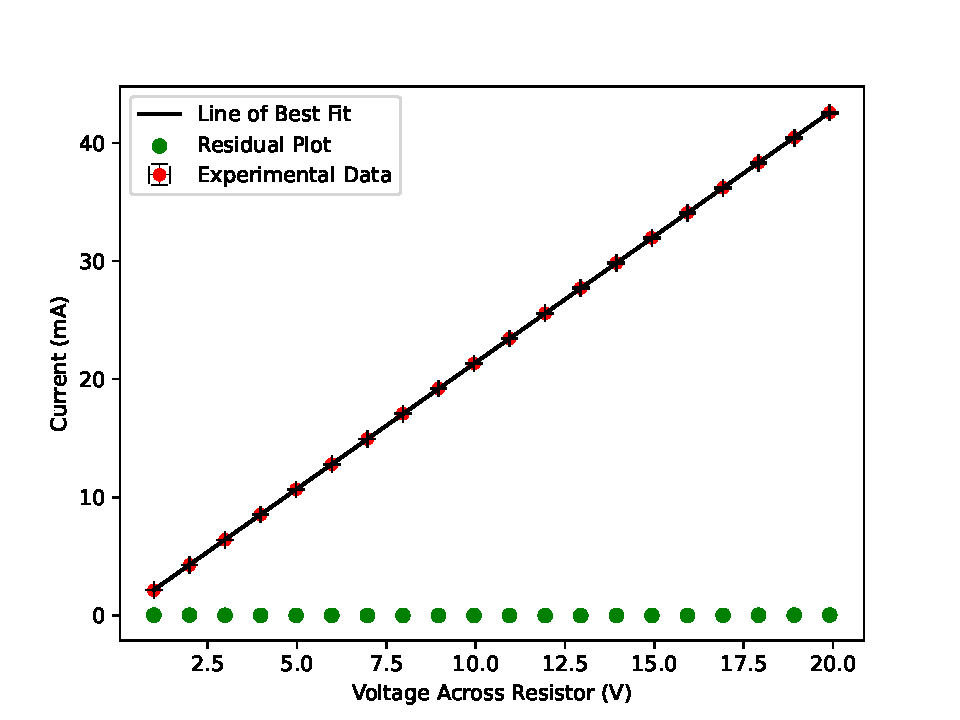
\includegraphics[width=0.75\textwidth]{experimentOne}[h]
\end{center}
\begin{center}
    \textbf{Figure 5.2: Experiment 2 Battery Voltage vs Current}
    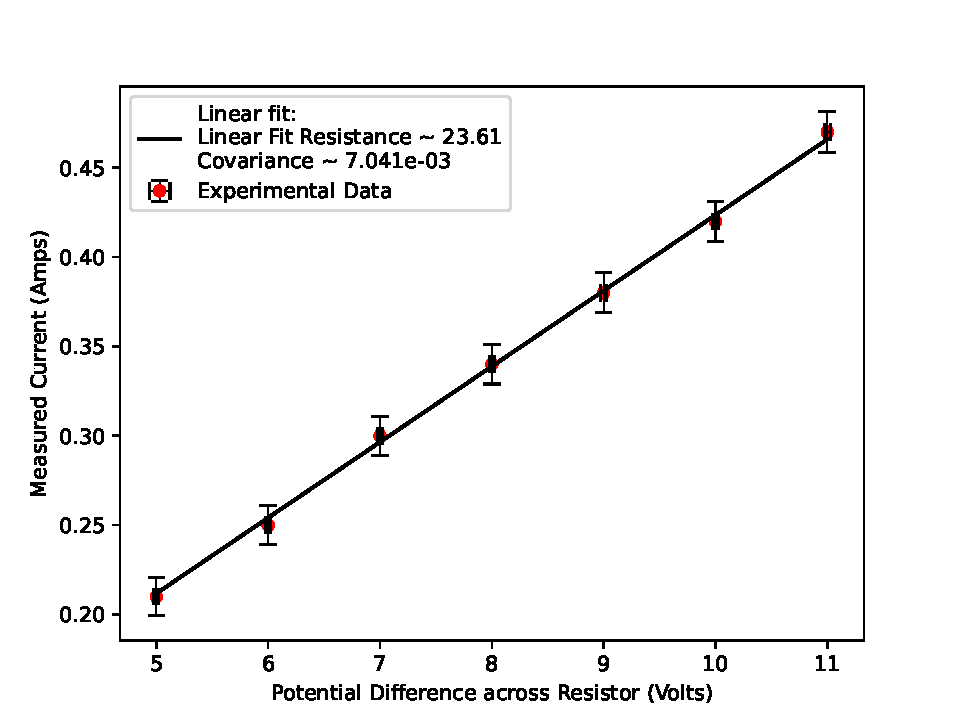
\includegraphics[width=0.75\textwidth]{experimentTwo}[h]
\end{center}
\begin{center}
    \textbf{Figure 5.3: Experiment 3 Battery Voltage vs Current}
    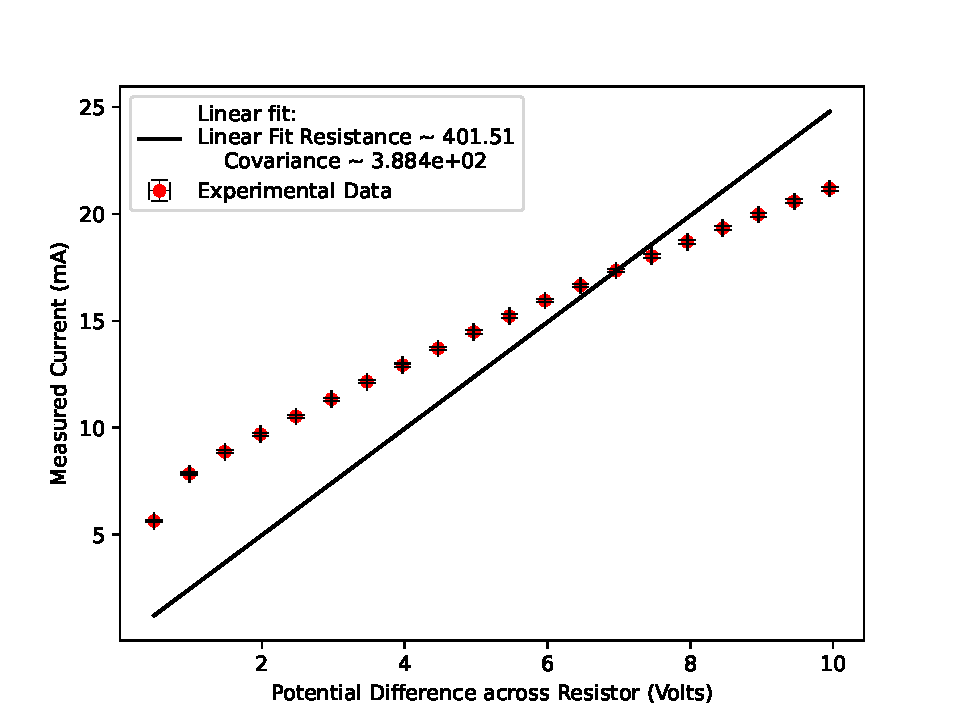
\includegraphics[width=0.75\textwidth]{experimentThree}[h]
\end{center}

\begin{center}
    \textbf{Figure 5.4: Ohm's Law python model used to generate best fit line}
\end{center}
\begin{verbatim}
    def current_model(voltage, resistance):
        return voltage / resistance
\end{verbatim}
{\large\textbf{Final Values}}\\

\textbf{Experiment 1}\\
The linear fit gave a value of $10.0\Omega$ for the first resistor.\\

\textbf{Experiment 2}\\
The linear fit gave a value of $23.5\Omega$ for the second resistor.\\

\textbf{Experiment 3}\\
The linear fit gave a value of $25.61\Omega$ for the net resistance.\\
The $R_{resistor}$ is the same as the resistor in experiment 2 which is a previously determined value. $R_{wire}$ can be calculated using the previously determined $R_{resistor}$ and $R_{net}$ calculated values as follows.
$$R_{net} = R_{wire} + R_{resistor} \implies R_{wire} = R_{net} - R_{resistor} = 25.6 - 23.5 = 2.1\Omega$$\\
Therefore the calculated resistance of the wire is $2.1\Omega$
\section{Discussion}
The first resistor has the following colours: Brown Black Black Gold. This corresponds to $10\times 10^0\Omega \pm 5\% = 10\Omega\pm0.5\Omega$. The experimentally calculated value was $10.0\Omega$, therefore the experiment was a completely accurate representation of Ohm's Law.\\

The second resistor had the following colours: Red Yellow Black Gold. This corresponds to $24\times10^0 \Omega \pm 5\% = 24\Omega\pm 1.2\Omega$. The experimentally calculated value was $23.6\Omega$, therefore the experimental value was within the uncertainty range of the resistor.\\

\end{document}